\documentclass[paper=a4, fontsize=11pt]{article} % A4 paper and 11pt font size
\usepackage[bottom=1.2in]{geometry}

\usepackage{amsmath,amsfonts,amsthm} % Math packages

\usepackage{graphicx}


\graphicspath{ {./figs/} }
%----------------------------------------------------------------------------------------
% TITLE SECTION
%----------------------------------------------------------------------------------------

\title{	Simulation of Pedestrian Movement Outside Football Stadium}

\author{Xiong Ding, Phani Teja Anumanchupallik, Wesley Hughes} % Your name

\date{\today} % Today's date or a custom date


%----------------------------------------------------------------------------------------
% content section
%----------------------------------------------------------------------------------------
\begin{document}

\maketitle % Print the title

\section{Problem Description}

\section{Literature review}

\section{Conceptual model}
Cellular automata divides the simulation domain into regular cells.
Each cell can be labeled as \textbf{allowed} or \textbf{forbidden} 
corresponding to the street and off-street area respectively. We 
build models for pedestrians and the floor and update the their
status based on the interaction between these two objects.

\subsection{Inputs}

In order to simulate the pedestrian flow outside Georgia Tech's Bobby Dodd Stadium,
we need some real physical data about the stadium, pedestrians and street configuration
around the stadium. Even though, variables like pedestrians' speed, 
space needed by people with different body sizes should vary individually, we use 
average value instead to simply our simulation.

\paragraph{Velocity} Follow reference ** and our own daily experience, we propose the
average pedestrian speed is $1.34 m/s$. 

\paragraph{Cellular space} Different people may occupy different size on the 
street. In order to take this fact into consideration, we take a square cellular 
configuration, in which each cell has edge length $0.3m$. And a pedestrian
who requires more space will have empty cells round them. We generate a distribution 
of the empty cells by each pedestrian.
\begin{equation}
  \label{eq:1}
  p(n) = e^{-\alpha n}
\end{equation}

\paragraph{Map construction}

\begin{figure}[h]
  \centering
  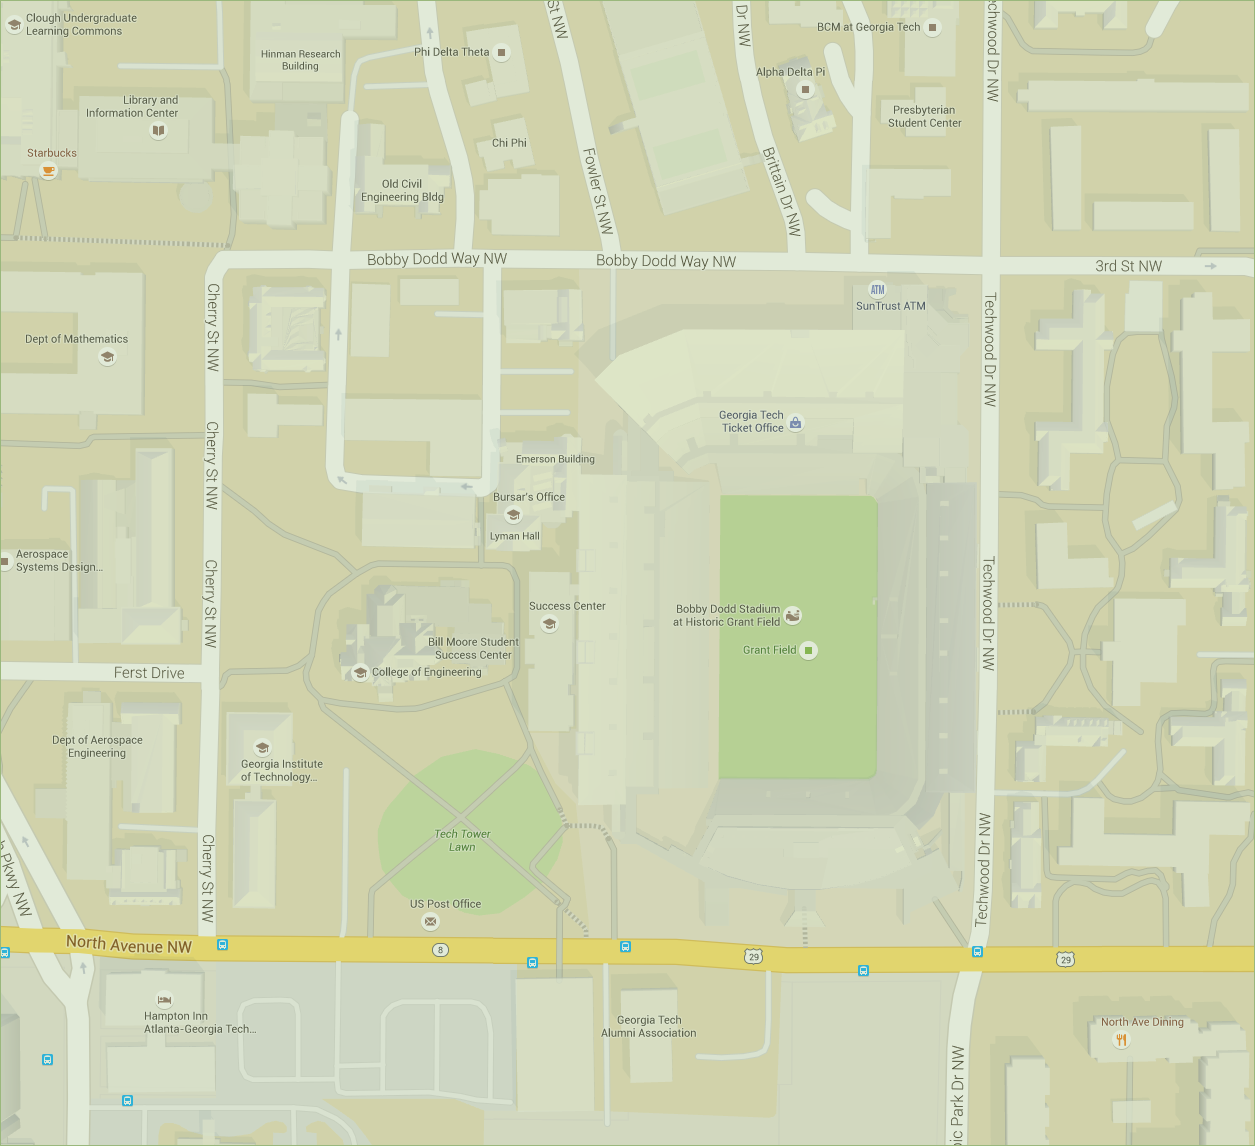
\includegraphics[width=0.4\textwidth]{map}
  \caption{Stadium area from Google Map.}
  \label{fig:map}
\end{figure}

The stadium area is shown in Fig.~\ref{fig:map}. Using Google Map distance
service, we get the west-east distance 483 meters and north-south distance
466 meters. [todo: insert a simplified map here]. The 4 main 
streets around the stadium has an average width 4.8 meters. So we use a 
$1610\times 1553$ matrix to represent the whole map and we set each street
has 16 cells along the transverse direction.


\paragraph{Space of each pedestrian} We know that different people may

\subsection{Outputs}

\subsection{simulation components and rules}

\paragraph{Floor model}
Static floor field: \\
dynamic floor field.\\
pedestrian field (transition matrix): Euclidean distance formula. \\
occupation matrix \\

\paragraph{Pedestrian model}
target variable \\
exit variable \\
group id (generator generates groups.) \\
happy/unhappy variable \\
consecutive jam time variable \\

\paragraph{Transition matrix}

\paragraph{Resolving conflicts}

\paragraph{update strategy}

%------------------------------------------------------------------------

\end{document}
